\documentclass[12pt,aspectratio=169,ignorenonframetext]{ltxbeamer}

\usepackage[spanish,es-nodecimaldot,es-tabla]{babel}
\usepackage{tabularx}

\title{El universo {\lmr\LaTeX}}
\subtitle{Curso de {\lmr\LaTeX}}
\author{Joar Buitrago\texorpdfstring{\thanks{jebuitragoc@unal.edu.co}}{ <jebuitragoc@unal.edu.co>}}
\date{}

\addbibresource{bibliography.bib}



\begin{document}
\begin{frame}
\maketitle
\end{frame}



\section{Contacto}
\begin{frame}
\begin{columns}
    \begin{column}{0.5\linewidth}
        \centering
        \includegraphics[width=0.75\linewidth]{assets/PillFall_QR.pdf}\par
        \vspace{0.05\linewidth}
        Joar Buitrago
    \end{column}

    \begin{column}{0.5\linewidth}
        \centering
        \includegraphics[width=0.75\linewidth]{assets/repository_QR.pdf}\par
        \vspace{0.05\linewidth}
        \href{https://github.com/PillFall/Curso-LaTeX}{github.com/PillFall/Curso-LaTeX}
    \end{column}
\end{columns}
\end{frame}



\section{Información del Curso}
\begin{frame}
\frametitle{Información del Curso}

\centering
\vfill

{\Large\bfseries Este curso está dividido en dos niveles de maestría.}\par\bigskip

\begin{tabular}{ccc}
    \textbf{Nivel I} & \textbf{Nivel II} \\
    \textit{Principiante} & \textit{Avanzado} \\
    \parbox{0.4\linewidth}{\centering\small Fundamentos y estructura.} &
    \parbox{0.4\linewidth}{\centering\small Diseño y Programación}
\end{tabular}

\vfill

\begin{alertblock}{Importante}
    Si usted considera que su nivel es más avanzado, por favor, inicie directamente en el nivel correspondiente.
\end{alertblock}
\end{frame}



\section{Un poco de historia}

\begin{frame}
\centering
\vfill
\resizebox{0.95\linewidth}{!}{\uncover<2->{¿}{\lmr\LaTeX}\uncover<2->{?}}
\vfill
\end{frame}



\begin{frame}
    \frametitle{¿De dónde viene todo esto?}

    \pause

    \begin{itemize}[<+->]
        \item \emph{1978 --- {\lmr\TeX}:} Donald Knuth crea {\lmr\TeX} frustrado por la baja calidad de las pruebas de imprenta de sus libros de computación.
        \item \emph{1984 --- {\lmr\LaTeX}:} Leslie Lamport desarrolla un conjunto de macros para que {\lmr\TeX} fuera más fácil de usar, separando el contenido del formato.
        \item \emph{Hoy:} Es mantenido por el \textit{{\lmr\LaTeX} Project Team} y es la herramienta estándar en el mundo académico.
    \end{itemize}
    \centering
    \vfill
    \uncover<+->{\emph{«LaTeX is a document preparation system for high-quality typesetting.»}}
\end{frame}



\section{¿Qué es {\lmr\LaTeX}?}
\begin{frame}
\frametitle{¿Qué es {\lmr\LaTeX}?}

\pause

{\lmr\LaTeX} es un sistema de composición de textos de calidad artística y tipográfica. Es usado muy habitualmente en el mundo científico debido a todas sus características y facilidad de trabajo.

\pause

{\lmr\LaTeX} es un conjunto de macros de {\lmr\TeX}, publicado bajo la licencia {\it{\lmr L}PPL}, {\it{\lmr\LaTeX} Project Public License}. Por lo cual es \emph{Software Libre} y gratuito.
\end{frame}



\begin{frame}
\frametitle{¿Qué es {\lmr\LaTeX}?}

\pause

\begin{itemize}[<+->]
    \item WYSIWYM
    \item Lenguaje de Programación
    \item Tipografía Avanzada
    \item Gráficos Avanzados
\end{itemize}
\end{frame}



\begin{frame}
\centering
\vfill
\resizebox{0.95\linewidth}{!}{\uncover<2->{¿}WYSIWYM\uncover<2->{?}}
\vfill
\end{frame}



\begin{frame}
\begin{columns}
    \begin{column}{0.5\linewidth}
        \raggedright
        \textbf{WYSIWYG}\par
        \vspace{0.3cm}
        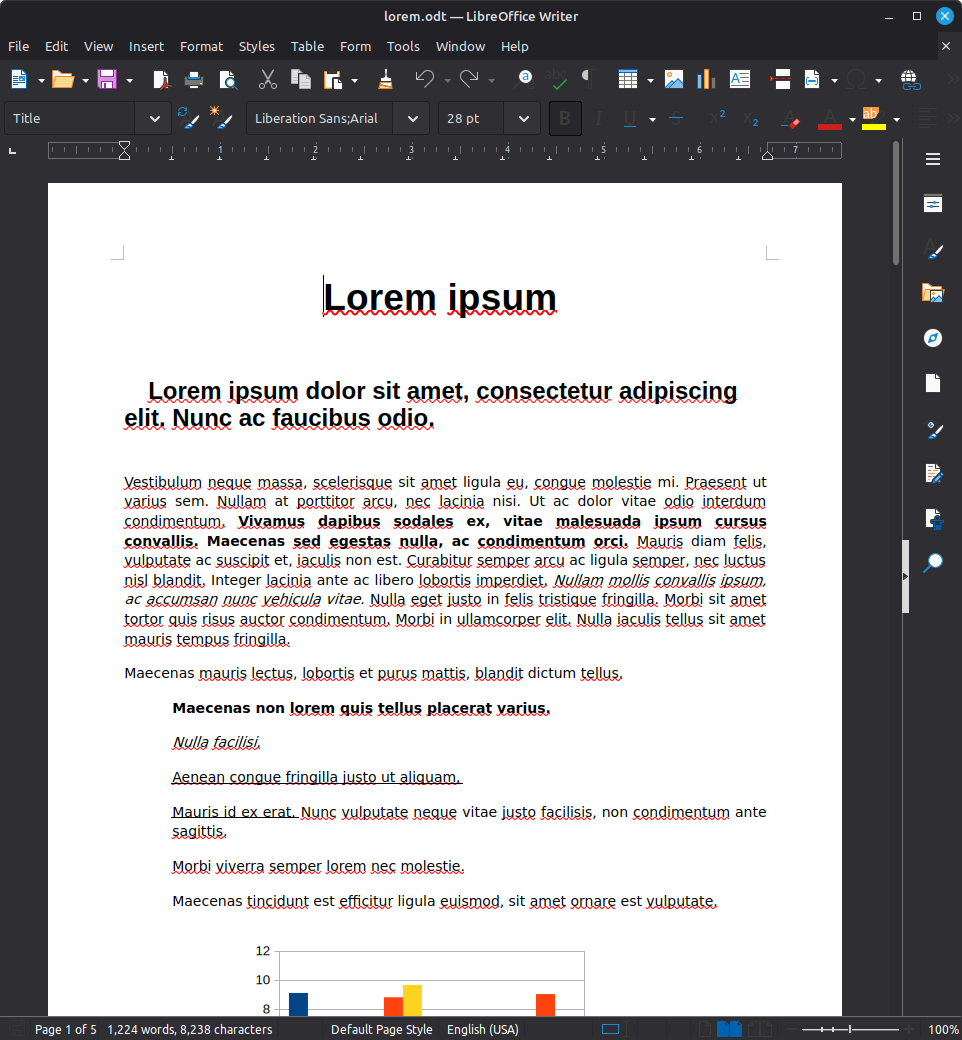
\includegraphics[width=0.95\linewidth]{assets/writer_screen.png}
    \end{column}
    \begin{column}{0.5\linewidth}
        \raggedleft
        \textbf{WYSIWYM}\par
        \vspace{0.3cm}
        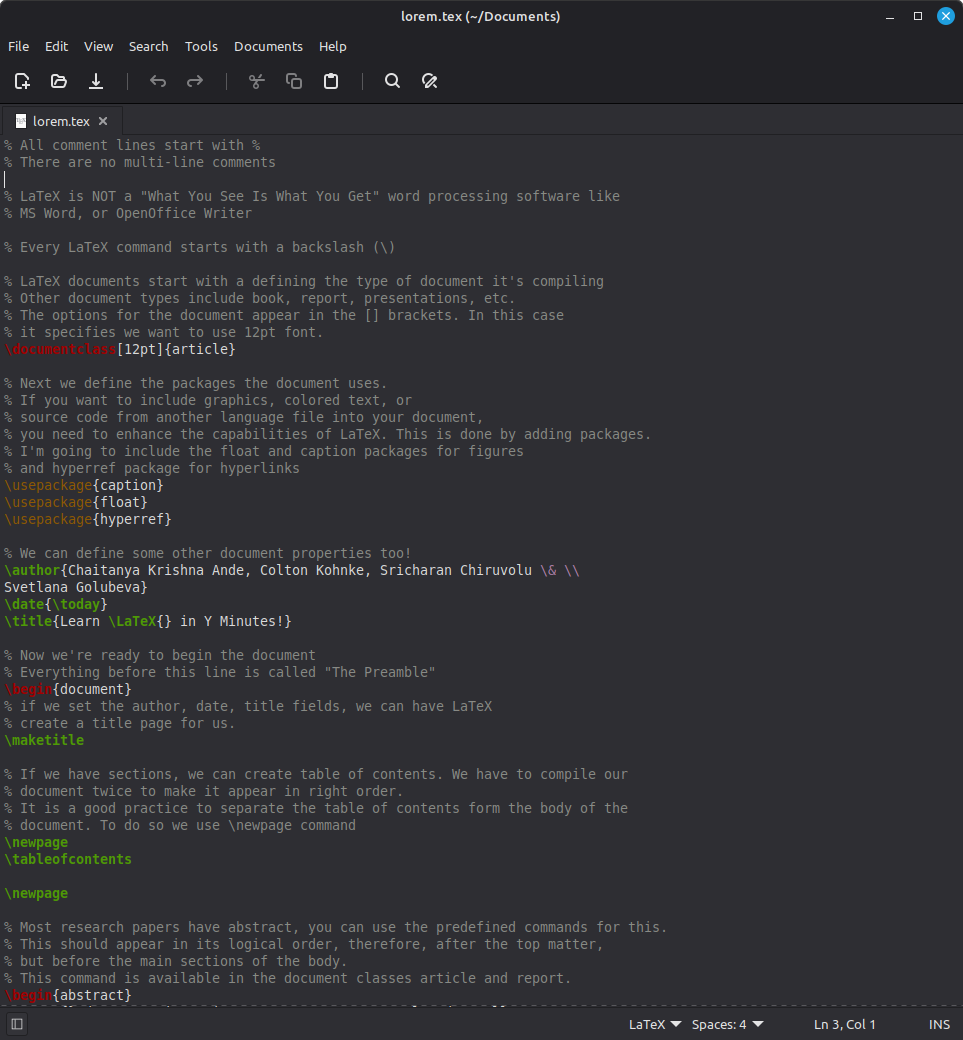
\includegraphics[width=0.95\linewidth]{assets/xed_screen.png}
    \end{column}
\end{columns}
\end{frame}


\begin{frame}
\begin{columns}
    \begin{column}{0.5\textwidth}
        \begingroup
        \centering \textbf{WYSIWYG}\\
        \textit{(What You See Is What You Get)}\\
        MS Word, Google Docs.\\
        \endgroup
        \vspace{0.3em}
        \begin{itemize}
            \item Formato visual inmediato.
            \item El autor se distrae con el diseño.
            \item Inestabilidad en documentos grandes.
        \end{itemize}
    \end{column}

    \begin{column}{0.5\textwidth}
        \centering \textbf{WYSIWYM}\\
        \textit{(What You See Is What You Mean)}\\
        {\lmr\LaTeX}, Markdown.\\
        \vspace{0.3em}
        \begin{itemize}
            \item El autor define la \textbf{estructura}.
            \item El sistema decide la \textbf{estética}.
            \item Formato ligero.
        \end{itemize}
    \end{column}
\end{columns}
\end{frame}



\begin{frame}[fragile]
\frametitle{Del Código al Papel}
\begin{columns}
    \begin{column}{0.45\textwidth}
        \begin{block}{Entrada (.tex)}
            \begin{minted}{latex}
\section{Física Moderna}
La energía en reposo es:
\begin{equation}
  E = mc^2 \label{eq:eins}
\end{equation}
Como vemos en (\ref{eq:eins})
            \end{minted}
        \end{block}
    \end{column}
    \pause

    \begin{column}{0.1\textwidth}
        \centering $\rightarrow$
    \end{column}

    \begin{column}{0.45\textwidth}
        \begin{exampleblock}{Salida (.dvi|.pdf)}
            \lmr
            \textbf{\Large 1. Física Moderna}\\
            \vspace{0.2cm}
            La energía en reposo es:
            \begin{equation*}
                E = mc^2 \quad (1)
            \end{equation*}
            Como vemos en (1)
        \end{exampleblock}
    \end{column}
\end{columns}
\end{frame}



\section{Pros y Contras}

\begin{frame}
\frametitle{¿Por qué sufrir con código?}
\begin{columns}
    \begin{column}{0.5\textwidth}
        \textbf{Ventajas:}
        \begin{itemize}
            \item Tipografía profesional (Kerning, ligaduras).
            \item Matemáticas perfectas.
            \item Gestión de bibliografía masiva.
            \item Automatización total de índices.
        \end{itemize}
    \end{column}

    \begin{column}{0.5\textwidth}
        \textbf{Desventajas:}
        \begin{itemize}
            \item Curva de aprendizaje inicial.
            \item El diseño de plantillas es complejo.
            \item No hay revisión visual instantánea.
        \end{itemize}
    \end{column}
\end{columns}
\end{frame}



\section{Motores y Distribuciones}

\begin{frame}
\frametitle{Motores y Distribuciones}
\begin{itemize}
    \item \textbf{Distribuciones:} TeX Live, MiKTeX, MacTeX (Mac).
    \item \textbf{Compiladores o Motores:}
    \begin{description}
        \item[\texttt{latex}] El original.
        \item[\texttt{pdflatex}] El estándar para pdf. (Deprecado).
        \item[\alert<2->{\texttt{xelatex}}] Ultrarápido.
        \item[\alert<2->{\texttt{lualatex}}] Con interpreté de Lua.
    \end{description}
\end{itemize}
\end{frame}



\section{Editores}

\begin{frame}
\frametitle{Editores}

{\lmr\LaTeX} es código, por lo que podremos usar cualquier editor de código o texto plano.

\pause

\begin{itemize}[<+->]
    \item Bloc de Notas
    \item VI
    \item Emacs
    \item Notepad++
    \item Visual Studio Code
\end{itemize}
\end{frame}

\begin{frame}
\frametitle{Editores}
\framesubtitle{IDE}

{\lmr\LaTeX} es código, por lo que podremos usar cualquier editor de código o texto plano.

Aunque lo ideal sería utilizar un Entorno de Desarrollo Integrado o editor especializado.

\pause

\begin{itemize}[<+->]
    \item {\lmr\raisebox{0.5ex}{\TeX}\fontshape{ui}\selectfont studio}
    \item {\lmr\TeX MAKER}
    \item {\lmr AUC\TeX}
    \item {\lmr L\kern-.125em\lower.5ex\hbox{Y}\kern-.125emX}
    \item Overleaf
\end{itemize}
\end{frame}



\section{Anatomía de un archivo \texttt{.tex}}
\begin{frame}[fragile]
\frametitle{Anatomía de un archivo \texttt{.tex}}

\pause

\begin{columns}
    \begin{column}{0.5\textwidth}

        \begin{minted}[escapeinside=||]{latex}
\documentclass[12pt]{article}|\tikz[remember picture,baseline]{\node [anchor=base] (class) {\strut};}|

\title{Mi Primer Documento}|\tikz[remember picture,baseline]{\node [anchor=base] (preamble begin) {\strut};}|
\author{Joar Buitrago}
\date{}|\tikz[remember picture,baseline]{\node [anchor=base] (preamble end) {\strut};}|

\begin{document}
\maketitle|\tikz[remember picture,baseline]{\node [anchor=base] (body begin) {\strut};}|
¡Hola, Mundo {\LaTeX}!|\tikz[remember picture,baseline]{\node [anchor=base] (body end) {\strut};}|
\end{document}
        \end{minted}
    \end{column}

    \begin{column}{0.5\textwidth}
        \tikz[remember picture,baseline]{\coordinate [anchor=base] (braces);}
    \end{column}
\end{columns}

\pause

\begin{tikzpicture}[remember picture, overlay]
    \draw [thick,decoration=brace,decorate] (class.north -| braces) -- (class.south -| braces) node [midway, right] {Clase};
    \draw [thick,decoration=brace,decorate] (preamble begin.north -| braces) -- (preamble end.south -| braces) node [midway, right] {Preámbulo};
    \draw [thick,decoration=brace,decorate] (body begin.north -| braces) -- (body end.south -| braces) node [midway, right] {Cuerpo};
\end{tikzpicture}
\end{frame}


\begin{frame}
\frametitle{Anatomía de un archivo \texttt{.tex}}
\framesubtitle{Clase}

La primera sección del documento, y la más corta es la \alert{clase del documento}.

\pause

En esta sección se define que tipo de documento se desea generar, junto con las opciones deseadas del mismo.
\end{frame}

\begin{frame}
\frametitle{Anatomía de un archivo \texttt{.tex}}
\framesubtitle{Clase}

{\lmr\LaTeX} define varias clases de documento entre las que se encuentran:

\begin{description}
    \item[{\bfseries\ttfamily article}] Se utiliza para la generación de artículos científicos, muchas clases personalizadas suelen extender esta.
    \item[{\bfseries\ttfamily report}] Se utiliza para la generación de reportes o escritos.
    \item[{\bfseries\ttfamily book}] Provee herramientas para la escritura de libros y otro tipo de documentos extensos, suele ser la clase en la que se realizan la mayoría los trabajos de grado.
    \item[{\bfseries\ttfamily letter}] Genera cartas y otro tipo de escritos cortos con un formato bastante formal, perfecto para documentos oficiales.
    \item[{\bfseries\ttfamily \only<1>{slides}\only<2->{\alert{beamer}}}] \only<1>{Presentaciones en diapositivas o acetatos}\only<2->{Presentaciones en pantallas o proyectores}
\end{description}
\end{frame}


\begin{frame}[fragile]
\frametitle{Anatomía de un archivo \texttt{.tex}}
\framesubtitle{Preámbulo}

La siguiente sección del documento que nos encontramos es el \alert{preámbulo}.

\pause

En esta sección se incluyen los paquetes que se desean utilizar, así como diversas instrucciones de configuración o personalización.

\pause

Hay instrucciones que solamente se pueden utilizar en el preámbulo.
\end{frame}



\begin{frame}
\frametitle{Anatomía de un archivo \texttt{.tex}}
\framesubtitle{Cuerpo}

La última sección del documento que nos encontramos es el \alert{cuerpo}.

\pause

En esta sección nos encontramos con el contenido de nuestro documento.

\pause

En esta sección {\lmr\LaTeX} procesa el documento en tres modos diferentes:
\end{frame}



\section{Estructura}


\subsection{Modos de procesamiento}
\begin{frame}
\frametitle{Modos de procesamiento}

\pause

\begin{description}[<+->]
    \item[Normal] El texto se separa en páginas, párrafos y renglones, se respetan las reglas gramaticales y de escritura.
    \item[ID] \emph{Izquierda a Derecha}, es similar al modo normal, pero {\lmr\LaTeX} asume que existe un solo renglón.
    \item[Matemático] Es similar al modo normal, excepto que todos los espacios son ignorados y se usan reglas de procesamiento matemático.
\end{description}
\end{frame}


\subsection{Espacio en blanco}
\begin{frame}[fragile]
\frametitle{Espacio en blanco}
\begin{columns}
    \begin{column}{0.45\textwidth}
        \begin{block}{Entrada (.tex)}
            \begin{minted}[linenos,xleftmargin=12pt]{latex}
In at auctor ex, eu
dictum lorem.
Morbi ut sem sed odio
ullam eleifend.

Cras tempor neque sapien.

Cras     auctor     sodales.
            \end{minted}
        \end{block}
    \end{column}
    \pause

    \begin{column}{0.1\textwidth}
        \centering $\rightarrow$
    \end{column}

    \begin{column}{0.45\textwidth}
        \begin{exampleblock}{Salida (.dvi|.pdf)}
            \setlength{\parskip}{\medskipamount}
            \lmr
            In at auctor ex, eu
            dictum lorem.
            Morbi ut sem sed odio
            ullam eleifend.

            Cras tempor neque sapien.

            Cras     auctor     sodales.
        \end{exampleblock}
    \end{column}
\end{columns}
\end{frame}



\subsection{Divisiones}
\begin{frame}[fragile]
\frametitle{Divisiones}

\begin{center}
    \begin{tabular}{ccc}
        \toprule
        División & Comando & Nivel \\
        \midrule
        Parte & \mintinline{latex}{\part} & -1 \\
        Capítulo & \mintinline{latex}{\chapter} & 0 \\
        Sección & \mintinline{latex}{\section} & 1 \\
        Subsección & \mintinline{latex}{\subsection} & 2 \\
        Sub-subsección & \mintinline{latex}{\subsubsection} & 3 \\
        Parágrafo & \mintinline{latex}{\paragraph} & 4 \\
        Sub-parágrafo & \mintinline{latex}{\subparagraph} & 5 \\
        \bottomrule
    \end{tabular}
\end{center}
\end{frame}



\begin{frame}[fragile]
\frametitle{Divisiones}

\begin{center}
    \begin{tabular}{ccc}
        \toprule
        División & Comando & Nivel \\
        \midrule
        Parte & \mintinline{latex}{\part*} & -1 \\
        Capítulo & \mintinline{latex}{\chapter*} & 0 \\
        Sección & \mintinline{latex}{\section*} & 1 \\
        Subsección & \mintinline{latex}{\subsection*} & 2 \\
        Sub-subsección & \mintinline{latex}{\subsubsection*} & 3 \\
        Parágrafo & \mintinline{latex}{\paragraph*} & 4 \\
        Sub-parágrafo & \mintinline{latex}{\subparagraph*} & 5 \\
        \bottomrule
    \end{tabular}
\end{center}
\end{frame}



\begin{frame}[fragile]
\frametitle{Divisiones}
\begin{columns}
    \begin{column}{0.45\textwidth}
        \begin{block}{Entrada (.tex)}
            \begin{minted}{latex}
\section{Física Moderna}
La energía en reposo es:
\begin{equation}
  E = mc^2
\end{equation}
            \end{minted}
        \end{block}
    \end{column}
    \pause

    \begin{column}{0.1\textwidth}
        \centering $\rightarrow$
    \end{column}

    \begin{column}{0.45\textwidth}
        \begin{exampleblock}{Salida (.dvi|.pdf)}
            \lmr
            \textbf{\Large 1. Física Moderna}\\
            \vspace{0.2cm}
            La energía en reposo es:
            \begin{equation*}
                E = mc^2 \quad (1)
            \end{equation*}
        \end{exampleblock}
    \end{column}
\end{columns}
\end{frame}


\begin{frame}[fragile]
\frametitle{Divisiones}
\begin{columns}
    \begin{column}{0.45\textwidth}
        \begin{block}{Entrada (.tex)}
            \begin{minted}{latex}
\section*{Física Moderna}
La energía en reposo es:
\begin{equation}
  E = mc^2
\end{equation}
            \end{minted}
        \end{block}
    \end{column}
    \pause

    \begin{column}{0.1\textwidth}
        \centering $\rightarrow$
    \end{column}

    \begin{column}{0.45\textwidth}
        \begin{exampleblock}{Salida (.dvi|.pdf)}
            \lmr
            \textbf{\Large Física Moderna}\\
            \vspace{0.2cm}
            La energía en reposo es:
            \begin{equation*}
                E = mc^2 \quad (1)
            \end{equation*}
        \end{exampleblock}
    \end{column}
\end{columns}
\end{frame}



\subsection{Referencias Cruzadas}
\begin{frame}[fragile]
\frametitle{Referencias Cruzadas}
\begin{columns}
    \begin{column}{0.45\textwidth}
        \begin{block}{Entrada (.tex)}
            \begin{minted}{latex}
\section{Física Moderna}
La energía en reposo es:
\begin{equation}
  E = mc^2 \label{eq:eine}
\end{equation}
Como se puede ver en (\ref{eq:eine})
            \end{minted}
        \end{block}
    \end{column}
    \pause

    \begin{column}{0.1\textwidth}
        \centering $\rightarrow$
    \end{column}

    \begin{column}{0.45\textwidth}
        \begin{exampleblock}{Salida (.dvi|.pdf)}
            \lmr
            \textbf{\Large 1. Física Moderna}\\
            \vspace{0.2cm}
            La energía en reposo es:
            \begin{equation*}
                E = mc^2 \quad (1)
            \end{equation*}
            Como se puede ver en (1)
        \end{exampleblock}
    \end{column}
\end{columns}
\end{frame}


\begin{frame}[fragile]
\frametitle{Referencias Cruzadas}
\begin{columns}
    \begin{column}{0.45\textwidth}
        \centering
        \mintinline{latex}{\label{patata}}
    \end{column}
    \pause

    \begin{column}{0.1\textwidth}
        \centering $\leftarrow$
    \end{column}

    \begin{column}{0.45\textwidth}
        \centering
        \mintinline{latex}{\ref{patata}}
    \end{column}
\end{columns}

\pause
\bigskip

\begin{columns}
    \begin{column}{0.45\textwidth}
        \centering
        \mintinline{python}{patata = current_label}
    \end{column}
    \pause

    \begin{column}{0.1\textwidth}
    \end{column}

    \begin{column}{0.45\textwidth}
        \centering
        \mintinline{python}{print(patata.number)}
    \end{column}
\end{columns}

\pause
\bigskip

\begin{columns}
    \begin{column}{0.45\textwidth}
        \centering
    \end{column}

    \begin{column}{0.1\textwidth}
    \end{column}

    \begin{column}{0.45\textwidth}
        \centering
        6
    \end{column}
\end{columns}
\end{frame}



\begin{frame}[fragile]
\frametitle{Referencias Cruzadas}
\begin{columns}
    \begin{column}{0.45\textwidth}
        \centering
        \mintinline{latex}{\label{potato}}
    \end{column}

    \begin{column}{0.1\textwidth}
        \centering $\leftarrow$
    \end{column}

    \begin{column}{0.45\textwidth}
        \centering
        \mintinline{latex}{\pageref{potato}}
    \end{column}
\end{columns}

\bigskip

\begin{columns}
    \begin{column}{0.45\textwidth}
        \centering
        \mintinline{python}{potato = current_label}
    \end{column}
    \pause

    \begin{column}{0.1\textwidth}
    \end{column}

    \begin{column}{0.45\textwidth}
        \centering
        \mintinline{python}{print(potato.page_number)}
    \end{column}
\end{columns}

\pause
\bigskip

\begin{columns}
    \begin{column}{0.45\textwidth}
        \centering
    \end{column}

    \begin{column}{0.1\textwidth}
    \end{column}

    \begin{column}{0.45\textwidth}
        \centering
        42
    \end{column}
\end{columns}
\end{frame}



\begin{frame}[fragile]
\frametitle{Referencias Cruzadas}
\begin{columns}
    \begin{column}{0.45\textwidth}
        \begin{minted}{latex}
\label{apple}

.
.
.

\label{apple}
        \end{minted}
    \end{column}

    \begin{column}{0.45\textwidth}
        \texttt{LaTeX Warning: There were multiply-defined labels.}
    \end{column}
\end{columns}
\end{frame}



\begin{frame}[fragile]
\frametitle{Referencias Cruzadas}
\begin{columns}
    \begin{column}{0.45\textwidth}
        \begin{minted}{latex}
\label{apple}

.
.
.

\label{apple}
        \end{minted}
    \end{column}

    \begin{column}{0.45\textwidth}
        \texttt{LaTeX Warning: There were multiply-defined labels.}
    \end{column}
\end{columns}
\end{frame}



\subsection{Referencias Cruzadas}
\begin{frame}[fragile]
\frametitle{Referencias Cruzadas}
\begin{columns}
    \begin{column}{0.45\textwidth}
        \begin{block}{Entrada (.tex)}
            \begin{minted}{latex}
\tableofcontents

.
.
.

\section{Historia}
\subsection{Clásica}
\subsection{Moderna}
\section{Ecuaciones}
            \end{minted}
        \end{block}
    \end{column}
    \pause

    \begin{column}{0.1\textwidth}
        \centering $\rightarrow$
    \end{column}

    \begin{column}{0.45\textwidth}
        \begin{exampleblock}{Salida (.dvi|.pdf)}
            \lmr
            \textbf{\Large Contenido}

            \medskip

            \begin{tabularx}{\linewidth}{rXr}
                1. & Historia & 2 \\
                & 1.1. Clásica & 3 \\
                & 1.2. Moderna & 10 \\
                2. & Ecuaciones & 15
            \end{tabularx}
        \end{exampleblock}
    \end{column}
\end{columns}
\end{frame}



\subsection{Paquete \texttt{hyperref}}
\begin{frame}[fragile]
\frametitle{Paquete \texttt{hyperref}}

La función más visible de \texttt{hyperref} es convertir referencias de texto en enlaces (o hipervínculos) totalmente funcionales dentro del PDF.

\begin{itemize}[<+->]
\item \textbf{Navegación Interna:}
    \begin{itemize}
    \item Entradas de (\mintinline{latex}{\tableofcontents}) interactivas.
    \item Las referencias cruzadas (\mintinline{latex}{\ref}) interactivas.
    \end{itemize}
\item \textbf{Enlaces Externos:}
    \begin{itemize}
    \item Enlaces interactivos: \mintinline{latex}{\url{dirección web}}.
    \item El texto se muestra como la dirección, y al hacer clic, se abre en el navegador.
    \end{itemize}
\end{itemize}
\end{frame}

\begin{frame}[fragile]
\frametitle{El comando \mintinline{latex}{\hypersetup{}}}

Los metadatos son información descriptiva (título, autor, palabras clave) que se «esconde» en el PDF.

Ayudan a que el archivo sea encontrado en buscadores o en el explorador de archivos.

\pause

\begin{minted}{latex}
\hypersetup{
    pdftitle={The TeXbook},
    pdfauthor={Donald Knuth},
    pdfkeywords={TeX, text processing, typesetting},
}
\end{minted}

\begin{alertblock}{Nota}
    Este comando solo puede usarse en el \emph{preámbulo}.
\end{alertblock}
\end{frame}



\begin{frame}[allowframebreaks]
\frametitle{Referencias}
\nocite{*}
\printbibliography
\end{frame}
\end{document}
